% Matteo Kumar
% PPB2 Solarzelle
%Grundlagen

\chapter{Grundlagen}
\section{Bändermodell und Halbleiter}
\subsection{Leitfähigkeit im Bändermodell}
Will man die Leitfähigkeit von Materialien anschaulich betrachten, ist das sog. Bändermodell hilfreich, das die erlaubten Energiezustände in einem Festkörper beschreibt. Jedes Band kann eine endliche Zahl an Ladungträgern enthalten; ist das Band voll besetzt, trägt es nicht zur Leitfähigkeit bei, da keine freien Energieniveaus existieren, um Energie aus einem elektrischen Feld aufzunhemen. Für die Leitfähigkeit wichtig sind vor allem das Valenzband und das Leitungsband. Das Leitungsband ist das energetisch niedrigste Band, das bei tiefen Temperaturen nicht voll besetzt ist; das Valenzband ist das unmittelbar darunter liegende Band. (Quelle: Eichler: Neues Phy GP S. 299f)
Elektrische Leiter haben bereits bei sehr niedrigen Temperaturen Ladungsträger im Leitungsband, weshalb sie i.Allg. immer leitend sind. Halbleiter und Isolatoren hingegen haben diese Eigenschaft nicht. Der Unterschied zwischen diesen beiden liegt in der Breite sog. Bandlücke, der energetische Abstand zwischen Valenz- und Leitungsband. Während die Bandlücke von Isolatoren sehr breit ist, ist die von Halbleitern hinreichend schmal, sodass bei geringen (z.B. thermischen) Energien Ladungsträger aus dem Valenz- in das Leitungsband wechseln können und so den Halbleiter leitend machen. \\
\begin{figure}[h]
    \centering
    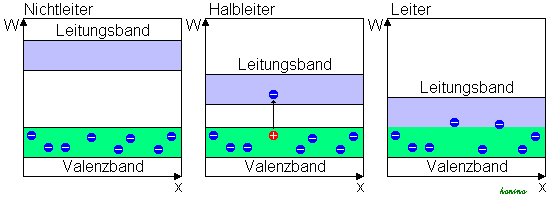
\includegraphics[scale=0.75]{Bilder/Baendermodell.png}
    \caption{Bändermodell für Nichtleiter, Halbleiter und Leiter \protect \footnotemark}
\end{figure}

\footnotetext{\url{https://www.virtualuniversity.ch/elektronik/analog/halbleiter/1.html}, Stand: 9.9.21}


\subsection{Dotierung von Halbleitern und pn-Übergang}
Die Leitfähigkeit von Halbleitern lässt sich durch Dotierungen verbessern. Man hat hierzu zwei Möglichkeiten: p- und n-Dotierung. \\
Bei der n-Dotierung werden Atome mit einem Valenzelektron mehr als die des Halbleitermaterials eingebracht. Dies hat zur Folge, dass das überschüssige Elektron bereits mit thermischen Energien in das Leitungsband angeregt werden kann. Die Leitfähigkeit wird erhöht und es bleibt ein positiv geladener Atomrumpf zurück.\\
Die p-Dotierung bedient sich des umgekehrten Prinzips. Das Halbleitermaterial wird mit einer Atomsorte mit einem Elektron weniger verunreinigt. Das Fehlelektron wird auch als "Loch" bezeichnet. Dieses Loch hat eine hohe Elektronenaffinität, weshalb es ein Elektron von einem Atom des Halbleiters bindet, das nun wiederum ein Loch hat. Diese Leitungsart wird auch als Lochleitung bezeichnet. Im Gegensatz zur n-Dotierung bleibt hier ein negativ geladener Atomrumpf zurück. (Quelle: H. Göbel, Einführung in die Halbleiter-Schaltungstechnik S. 7-11). Bei einer Dotierung verschiebt sich auch die Fermienergie, die im Falle eines undotierten Leiters ungefähr in der Mitte zwischen Unterkante des Leitungsbandes und Oberkante des Valenzbandes liegt. Im Falle einer n-Dotierung verschiebt sich die Fermienergie aufgrund der zusätzlichen Elektronen im Valenzband nach oben, im Falle einer p-Dotierung aufgrund der zusätzlichen Löcher nach unten. (Quelle: P: Wellmann, Halbleiter, S.60)\\
Fügt man nun einen p- und einen n-dotierten Halbleiter zusammen, erhält man einen sogenannten pn-Übergang. Im p-dotierten Halbleiter herrscht ein Löcherüberschuss und im n-dotierten ein Elektronenüberschuss. Aufgrund dieses Konzentrationsgefälles wandern Elektronen und Löcher und rekombinieren, bis sich ein Gleichgewicht einstellt. Nun existiert direkt am Übergang zwischen den Materialien eine Zone, in der es keine freien Ladungsträger mehr gibt. Es liegen nur noch die negativ bzw. positiv geladenen Atomrümpfe vor, die ihrerseits wieder eine Potentialdifferenz verursachen.\\
Legt man nun ein externes Feld an, kann, je nach Anlegrichtung, diese Differenz entweder vergrößert werden und es fließt kein Strom, die Sperrzone vergrößert sich, oder sie wird verringert bis sie schließlich überwunden wird. Es existiert ein Stromfluss. \\
Dies kann auch im Bändermodell betrachtet werden: Durch die Rekombination von freien Löchern und Elektronen in der Verarmungszone gleichen sich die Fermienergien beider Materialien an. Dabei verbiegt sich das Band und es entsteht eine Potentialdifferenz zwischen p- und n-dotiertem Halbleiter. \\

\begin{figure}[h]
    \centering
    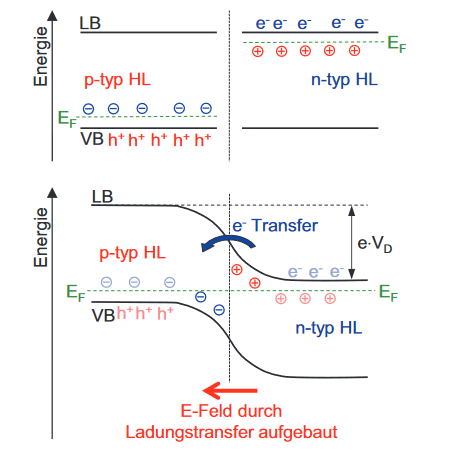
\includegraphics[scale=0.5]{Bilder/Bandverbiegung.png}
    \caption{Bei einem pn-Übergang gleichen sich die Fermienergien (in grün) an. Dadurch verbiegt sich das Band und es entsteht eine Potentialdifferenz}
\end{figure}

Quelle: Wellmann, S.62

\section{Solarzelle}
\subsection{Funktionsweise}
Der Typ von Solarzelle, mit dem sich in diesem Versuch beschäftigt wird, besteht im Wesentlichen aus einem pn-Übergang. Trifft nun Licht, also Photonen, auf die Zelle, werden dadurch freie Elektronen-Löcher-Paare erzeugt. Im einfachsten Fall werden diese Durch den Drift des elektrischen Feldes der Atomrümpfe in der Verarmungszone separiert und wandern in Richtung der aufgebrachten Kontakte; ein Strom kann abgegriffen werden. Manche Zellen nutzen zusätzlich noch die durch die Konzentrationsgefälle der Elektronen und Löcher bedingte Diffusion. (Quelle: Solar Cells and Modules, A.Shah, S.46) Unbeleuchtete Solarzellen unterscheiden sich also im prinzipiellen Aufbau nicht von einfachen Dioden; entsprechend stimmt auch der Verlauf ihrer U/I-Kennlinien überein. Wird die Zelle nun beleuchtet, bedingen die entstehenden Elektron-Löcher-Paare einen Kurzschlussstrom; die Kennlinie verschiebt sich im Vergleich zur Diode in negative I-Richtung. \\

\begin{figure}[h]
    \centering
    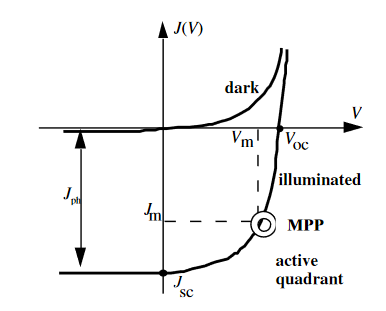
\includegraphics[scale=0.75]{Bilder/Kennlinien.png}
    \caption{U/I-Kennlinie einer Solarzelle für den beleuchteten und unbeleuchteten Fall}
    \label{bild:kennlinien}
\end{figure}

Quelle: Shah, S.50

\subsection{Ersatzschaltbild}
Die ideale Solarzelle kann durch eine Stromquelle, die den Photostrom modelliert, und eine Diode dargestellt werden. 
Erweitert werden kann dieses Modell durch einen Serienwiderstand, der hauptsächlich Widerstände in den Kontakten und Verkabelungen
widerspiegelt, und einen Parallelwiderstand, der alle Effekte im Kristall zusammenfasst, die den pn-Übergang überbrücken.
Quelle: Shah, S.52f 
Das Ersatzschaltbild in Abb. \ref{bild:ersatzschaltbild} zu finden.

\begin{figure}[h]
    \centering
    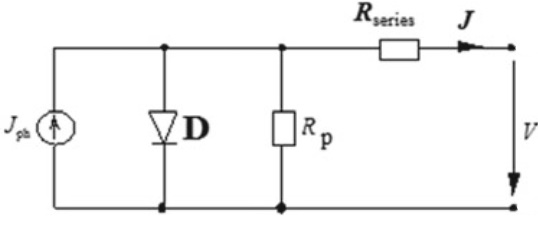
\includegraphics[scale=0.5]{Bilder/Ersatzschaltbild.png}
    \caption{Ersatzschaltbild einer Solarzelle}
    \label{bild:ersatzschaltbild}
\end{figure}
Quelle: Shah, S.53

Die sich daraus ergebende U/I-Kennlinie wird durch die Shockley-Gleichung beschrieben:
\begin{equation}
    I = I_0 (exp(\frac{q(U-R_SI)}{nkT})-1) + \frac{U-R_SI}{R_P} - I_{Ph}
\end{equation}

Quelle: Skript S.3

\subsection{Wichtige Kenngrößen}
Die Leistung berechnet sich nach $P = |UI|$, im U/I-Diagramm entspricht ihr also die Fläche des Rechtecks unter der Kennlinie. Am Maximum-Power-Point $MPP$ ist $P$ maximal. Der $MPP$ ist auch in Abb. \ref{bild:kennlinien} eingezeichnet. \\
Der Wirkungsgrad einer Solarzelle berechnet sich aus dem Verhältnis der nutzbaren und der einfallenden Leistung:
\begin{equation*}
\eta = \frac{P_{MPP}}{P_{ein}} = \frac{|UI|_{MPP}}{P_{ein}}
\end{equation*}
Ein weiterer Gütefaktor einer Solarzelle ist der Füllfaktor $FF$. Er ist das Verhältnis der Leistung am $MPP$ und des Produktes aus Leerlaufspannung $U_{OC}$ und Kurzschlussstrom $I_{SC}$. Eine ideale Solarzelle hat den Füllfaktor $1$, eine reale $FF < 1$.

\begin{equation*}
FF = \frac{|UI|_{MPP}}{U_{OC} I_{SC}}
\end{equation*}
Die Externe Quanteneffizienz $EQE$ einer Solarzelle beschreibt das Verhältnis von Photonen, die zum Photostrom beitragen, zu einfallenden Photonen. Man kann sie also auch als Wirkungsgrad bezogen auf Photonen betrachten; im Idealfall gilt $EQE = 1$. Es folgt:

\begin{equation}
EQE = \frac{Photonen \, im \, Photostrom}{einfallende \, Photonen} = \frac{ \frac{I_{Ph}t}{e}}{r_{ein}t} = \frac{I_{Ph}}{e \, r_{ein}} = \frac{I_{Ph} h \nu}{e P_\lambda}
\end{equation}

wobei im letzten Schritt angenommen wurde, dass das einfallende Licht monochromatisch ist, und $P_\lambda$ die einfallende Strahlungsleistung ist. \\
Schreibt man nun die Frequenz in die Wellenlänge um, erhält man:

\begin{equation}
EQE = \frac{h c}{e} \frac{I_{Ph}}{\lambda P_\lambda} = \frac{h c}{e} \frac{SE(\lambda)}{\lambda}
\end{equation}

Im letzten Schritt wurde hierbei ausgenutzt, dass der Vorfaktor konstant ist, um die Spektrale Empfindlichkeit $SE(\lambda) = \frac{I_{Ph}}{P_\lambda}$ zu definieren.

\subsection{Im Versuch verwendete Solarzelltypen}
Der Unterschied zwischen den im Versuch vorliegenden Silizium- und Kupfer-Indium-Selenoid-(CIS-)Zellen liegt in der Art der Bandlücke der jeweiligen Materialien. CIS-Zellen haben eine sogenannte direkte Bandlücke; auftreffende Photonen können direkt absorbiert werden. Dagegen haben Siliziumzellen eine indirekte Bandlücke; Photonen können erst durch eine Interaktion mit einem geeigneten Phonon absorbiert werden, weshalb die Absorptionswahrscheinlichkeit im Vergleich zur CIS-Zelle deutlich herabgesetzt ist. Aufgrund dessen sind bei Siliziumzellen wesentlich dickere Halbleiterschichten oder spezielle Lichtfallen nötig, um die Stromausbeute zu erhöhen (Quelle: Solar Cells and Modules, A.Shah, S.40). \\
Des Weiteren werden im Versuch zwei verschiedene Arten von Siliziumzellen verwende: Mono- und multikristalline. Monokristalline Solarzellen bestehen aus einem einzigen gewachsenem Kristall, im Gegensatz zu polykristallinen Solarzellen. Die Herstellung von Einkristallen ist zwar wesentlich aufwändiger und kostenintensiver, jedoch kann das Solarmodul bei Verwendung dieser einen deutlich höheren Wirkungsgrad erzielen. (Quelle: C. Altekrüger, S.26ff)
